\documentclass[10pt, a4paper]{beamer}
%\documentclass{article}

%Metadaten
\title{Machine Vision with Arduino Portenta H7}

\subtitle{Getting Started With the Portenta Vision Shield Camera}
%\institution{University of Applied Science Hochschule Emden/Leer}
\author{Vijay Singh}
%\date{\today}
\date{\today}

% siehe hesader.tex Zeile 10-16 zum Aktivieren der Notes
% Kommentare stehen in \notes{} und können im 2-screen-mode genutzt werden
%%%%%%
%
% $Autor: Wings $
% $Datum: 2020-01-18 11:15:45Z $
% $Pfad: githubtemplate/Template/Presentations/Template/slides/header.tex $
% $Version: 4620 $
%
%
% !TeX encoding = utf8
% !TeX root = Rename
%
%%%%%%


%Packages
\usepackage[utf8]{inputenc} %Für Umlaute, da BibLaTeX
\usepackage[german]{babel}
\usepackage{amsmath}
\usepackage{amsfonts}
\usepackage{amssymb}
\usepackage{colortbl}
\usepackage{cancel} %'\cancel{}', '\bcancel{}' und '\xcancel{}'

%%%%%%%%%2-Screen%%%%%%%%%%%%%%%%%%%%%%%%%%%%%%%%%%%%%%%%%%%%
\usepackage{pgfpages} 
%%%%Kommentiert für Beamer
%%%%Aktiv für Notes
%\setbeameroption{show notes on second screen=bottom}
%\setbeameroption{second mode text on second screen=bottom}
%%%%%%%%%%%%%%%%%%%%%%%%%%%%%%%%%%%%%%%%%%%%%%%%%%%%%%%%%%%%%

%Für Grafiken
\usepackage{tikz}
\usetikzlibrary{mindmap}
\usepackage{gnuplottex}
\usepackage{pgf}
\usepackage{colortbl} 
\usetikzlibrary{calc}
\usetikzlibrary{shapes,arrows} %Für Flowchart
\usetikzlibrary{shapes.geometric} %Für Flowchart
\usepackage{scalefnt}
\usetikzlibrary{decorations.markings} %Für => pfeile
\usetikzlibrary{calc,patterns,decorations.pathmorphing,decorations.markings}
%Für urls in Quellen
\usepackage{url}
%Für Diagramme (autotools)
%\usepackage{graphicx}
%\usepackage{graphviz}

%\usepackage[
%  backend=biber,
%  style=alphabetic,
%  sorting=ynt
%]{biblatex}

\usepackage[natbib=true,style=alphabetic,backend=bibtex,useprefix=true]{biblatex}

%Formatierungen
\mode<presentation>
\setbeamertemplate{headline} 
{%
\begin{beamercolorbox}[rounded=true, center]{bgcolor}
\begin{columns}[T]
\begin{column}{9cm}
{\color{gray}\begin{tiny}Hochschule Emden/Leer\end{tiny}} \\ 
{\color{gray}\begin{tiny}Department of Electrical and Computer Engineering\end{tiny}} \\ 
{\color{gray}\begin{tiny}Industrial Informatics\end{tiny}} \\
%{\color{gray}\begin{tiny}Innovationsforum MSR\end{tiny}}
\end{column}
\begin{column}{2cm}

\includegraphics[scale=0.25]{img/technik.jpg}
\end{column}
\end{columns}
\end{beamercolorbox}
 }
\insertsectionhead
\insertsubsectionhead
\usetheme{default}
\useinnertheme[shadow=true]{rounded}
\usebackgroundtemplate
{%
      \rule{0pt}{\paperheight}%
      \hspace*{\paperwidth}%
      \makebox[0pt][r]{
\includegraphics[width=\paperwidth]{img/hintergrund2.png}}
 }

\definecolor{HSELhellblau}{RGB}{138,198,203}
\definecolor{HSELblau}{RGB}{0,59,95}
\usecolortheme[named=HSELblau]{structure}
 \newcommand{\topline}{%
  \tikz[remember picture,overlay] {%
    \draw[HSELhellblau] ([yshift=-0.9cm]current page.north west)
             -- ([yshift=-0.9cm,xshift=\paperwidth]current page.north west);}}
\setbeamertemplate{section}[numbered]


\newcommand{\STANDARD}[2]
{
  \mode<presentation>%
  {%
     \begin{frame}[allowframebreaks]{#1} #2 \end{frame}
  }%
  \mode<article>
  {
    \fcolorbox{AliceBlue}%{Bisque} %{BlanchedAlmond}
    {LightGrey} %{Beige}   %{AliceBlue}
    {
      \begin{minipage}{\textwidth}{\bf #1} #2  \end{minipage}
      
      
    }%
    
    \medskip
    \hrulefill
  }
}

\newcommand{\MYNOTE}[1]
{
  \mode<presentation>%
  {%
     %\note{#1}
     \only<article>{#1}
  }%
  \mode<article>
  {
    #1
  }
}

% ------------
% sectionframe
% ------------
%
% #1  Der Name der section.
%
\newcommand{\sectionframe}[1]%
{%
	\begin{frame}
		\Huge
		\begin{center}
			#1 
		\end{center}
	\end{frame}%
}

\newcommand{\Mysection}[1]%
{%
  \section{#1}%
  
  \sectionframe{#1}%
}

\usepackage{listings}

% Farben für Syntax-Highlighting
\definecolor{dkgreen}{rgb}{0,.6,0}
\definecolor{dkblue}{rgb}{0.655,0.113,.364}
\definecolor{dkyellow}{cmyk}{0,0,.8,.3}

\definecolor{parameterc}{rgb}{.4,0,.6}
\definecolor{typec}{rgb}{0,0.525,.702}
\definecolor{stringc}{rgb}{0,.5019,.5019}
\definecolor{keywordc}{rgb}{.6549, .1137, .3647}
\definecolor{commentc}{rgb}{.5882, .5960, .5882}
\definecolor{textc}{rgb}{.2,.2,.2}

\lstdefinestyle{all}{
	alsoletter={-},
	frame=single, 	% top,frame=bottom,
	numbers=none,
	numberstyle=\tiny\color{textc},
	basicstyle=\linespread{0.9}\ttfamily\footnotesize\color{textc},
	tabsize=4,
	showstringspaces=false,
	captionpos=t,
	rulecolor=\color{lightgray!40},
	keywordstyle=\color{keywordc},
	stringstyle=\color{stringc},
	commentstyle=\color{commentc},
	breaklines=true,
	escapechar="!",
	postbreak=\mbox{\textcolor{green}{$\hookrightarrow$}\space},
}

\lstdefinestyle{bashstyle}{
	style=all,
	keywords=[2]{-y, --no-install-recommends, --allow-change-held-packages, --allow-downgrades, --fetch-keys, -n, --version, --params, -c, -i, -O, --upgrade, --no-cache-dir, --extra-index-url, --show, -s, -m},
	keywordstyle=[2]\color{parameterc},
	morekeywords = {ln,choco,pip,pip3,apt,apt-key,apt-get,apt-mark,add-apt-repository,wget,mktemp,dpkg,dpkg-query,echo,>>,rm,tegrastats, systemctl},
	deletekeywords={local,LOCAL},
}

\lstdefinestyle{pythonstyle}{
	style=all,
	morekeywords={as},
	keywords=[2]{True, False, None},
	keywordstyle=[2]\color{typec},
	alsoletter={_},
	keywords=[3]{max_workspace_size_bytes, precision_mode, maximum_cached_engines, use_calibration, optimizer, loss, input_shape, from_logits, metrics, batch_size, epochs, validation_data, activation, use_calibration, filters, kernel_size, pool_size, units},
	keywordstyle=[3]\color{parameterc},
	deletekeywords={compile,COMPILE},
}

\lstdefinestyle{inlinestyle}{
	style=all,
	breaklines        = true,
	breakatwhitespace = true,
	breakindent       = 2ex,
	escapechar        = *,
	numbers           = left,
	postbreak=,
}
\lstdefinelanguage{MyBash} {
	language = Bash,
	style=bashstyle,
}

\lstdefinelanguage{MyPython} {
	language = Python,
	style=pythonstyle,
}


\definecolor{PythonColor}{rgb}{0,0.5,1.}
\newcommand{\PYTHON}[1]{\textcolor{PythonColor}{\texttt{#1}}}
\definecolor{PythonColorHighLite}{rgb}{0.5,0,1.}
\newcommand{\PYTHONHL}[1]{\textcolor{PythonColorHighLite}{\texttt{#1}}}
\definecolor{MapleColor}{rgb}{1,0,0}
\newcommand{\MapleCommand}[1]{\textcolor{MapleColor}{\texttt{#1}}}
\definecolor{ShellColor}{rgb}{0,1,1.}
\newcommand{\SHELL}[1]{\textcolor{ShellColor}{\texttt{#1}}}
\definecolor{FileColor}{rgb}{1,0,1.}
\newcommand{\FILE}[1]{\textcolor{FileColor}{\texttt{#1}}}

%\addbibresource{Documents/MyLiterature.bib} %Import the bibliography file

\usepackage{listings}
\usepackage{xcolor}

\lstset{
	basicstyle=\ttfamily\small,
	keywordstyle=\color{blue},
	commentstyle=\color{gray},
	stringstyle=\color{red},
	numberstyle=\tiny\color{gray},
	stepnumber=1,
	numbersep=10pt,
	backgroundcolor=\color{white},
	showspaces=false,
	showstringspaces=false,
	breaklines=true,
	frame=single,
	tabsize=2,
	captionpos=b
}


\begin{document}
	
	
\setbeamercolor{bgcolor}{fg=black,bg=white}
\selectlanguage{german}
\setbeamertemplate{footline}{%
\vspace*{-.1cm}\hspace*{.5cm}
\scriptsize{%
%%\hspace*{1pt}\insertauthor
%%\inserttitle
\hspace{325pt}\insertframenumber/\inserttotalframenumber}
}

\STANDARD{}
{
  \titlepage
}

\MYNOTE
{
  \ldots
}



\STANDARD{}
{
\tableofcontents[hideallsubsections]
}

\MYNOTE
{
  \ldots
}

\setbeamercovered{transparent}
	
	\section{Overview}
	\begin{frame}
		\frametitle{Introduction}
		
		\begin{block}{}
			This presentation shows you how to capture frames from the \textbf{Arduino Portenta Vision Shield Camera module} and visualize the video output through a \textbf{Processing sketch.}
		\end{block}
		
		
		\begin{block}{Objectives}
			\begin{itemize}
				\item Capturing the frames from the camera
				\item Sending the frames as a byte stream through a Serial connection.
				\item Visualising the frames in Processing
			\end{itemize}
		\end{block}
		
		\begin{block}{Importance}
			Real-time object detection has applications in surveillance, industrial automation, robotics, and IoT, among others.
		\end{block}
		
		
	\end{frame}
	
	\section{Components}
	\begin{frame}
		\frametitle{Required Hardware and Software}
		
		\begin{block}{Description}
			The project involves the following components:
			\begin{itemize}
				\item \textbf{Arduino Portenta H7:} The core microcontroller unit providing processing power and resources for boarding different shields.
				\item \textbf{Portenta Vision Shield:} An accessory for the Portenta H7, equipped with a camera module and display for image capture and processing.
				\item \textbf{USB-C cable:} A pre-trained model deployed on the Portenta H7 for object detection tasks.
				\item \textbf{Arduino IDE:} A arduino software to capture the image data by the onboard camera.
				\item \textbf{Processing:} A processing software helps to visualize the data
			\end{itemize}
		\end{block}
		
	\end{frame}
	
	\begin{frame}
		
		\begin{block}{Instructions:}
			Accessing the Portenta Vision Shield's camera data is done with the help of both Arduino and the Processing IDE. The Arduino sketch handles the capture of image data by the on-board camera, while the java applet created with Processing helps to visualize this data with the help of a serial connection. The following steps will run you through how to capture, package the data through the serial port and visualize the output in Processing.
		\end{block}
		
	\end{frame}
	
	\begin{frame}
		\frametitle{Figures}
		
		\begin{columns}
			\column{0.5\textwidth}
			\centering
			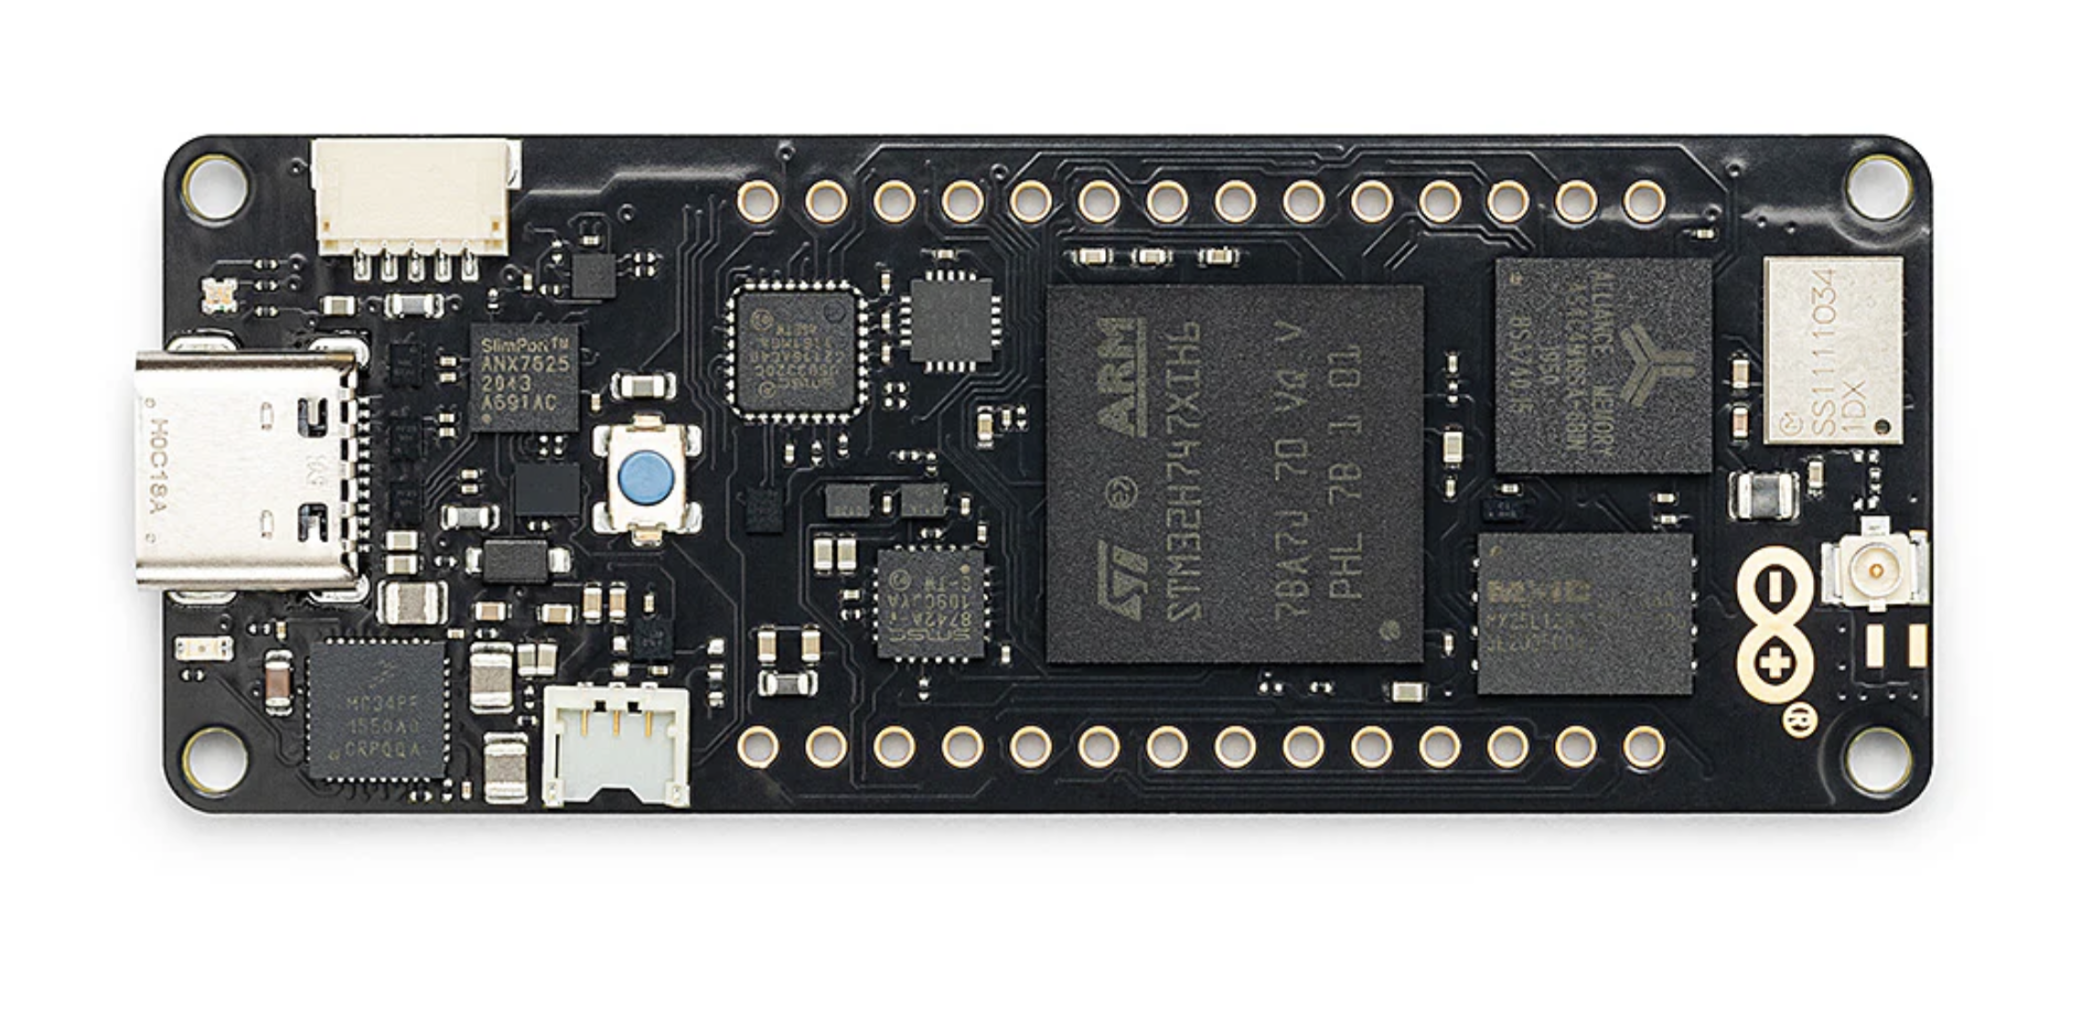
\includegraphics[width=\textwidth]{images/ArduinoPortentaH7.png}
			\vspace{0.2cm}
			\textbf{Figure1: Arduino PortentaH7}
			
			\column{0.5\textwidth}
			\centering
			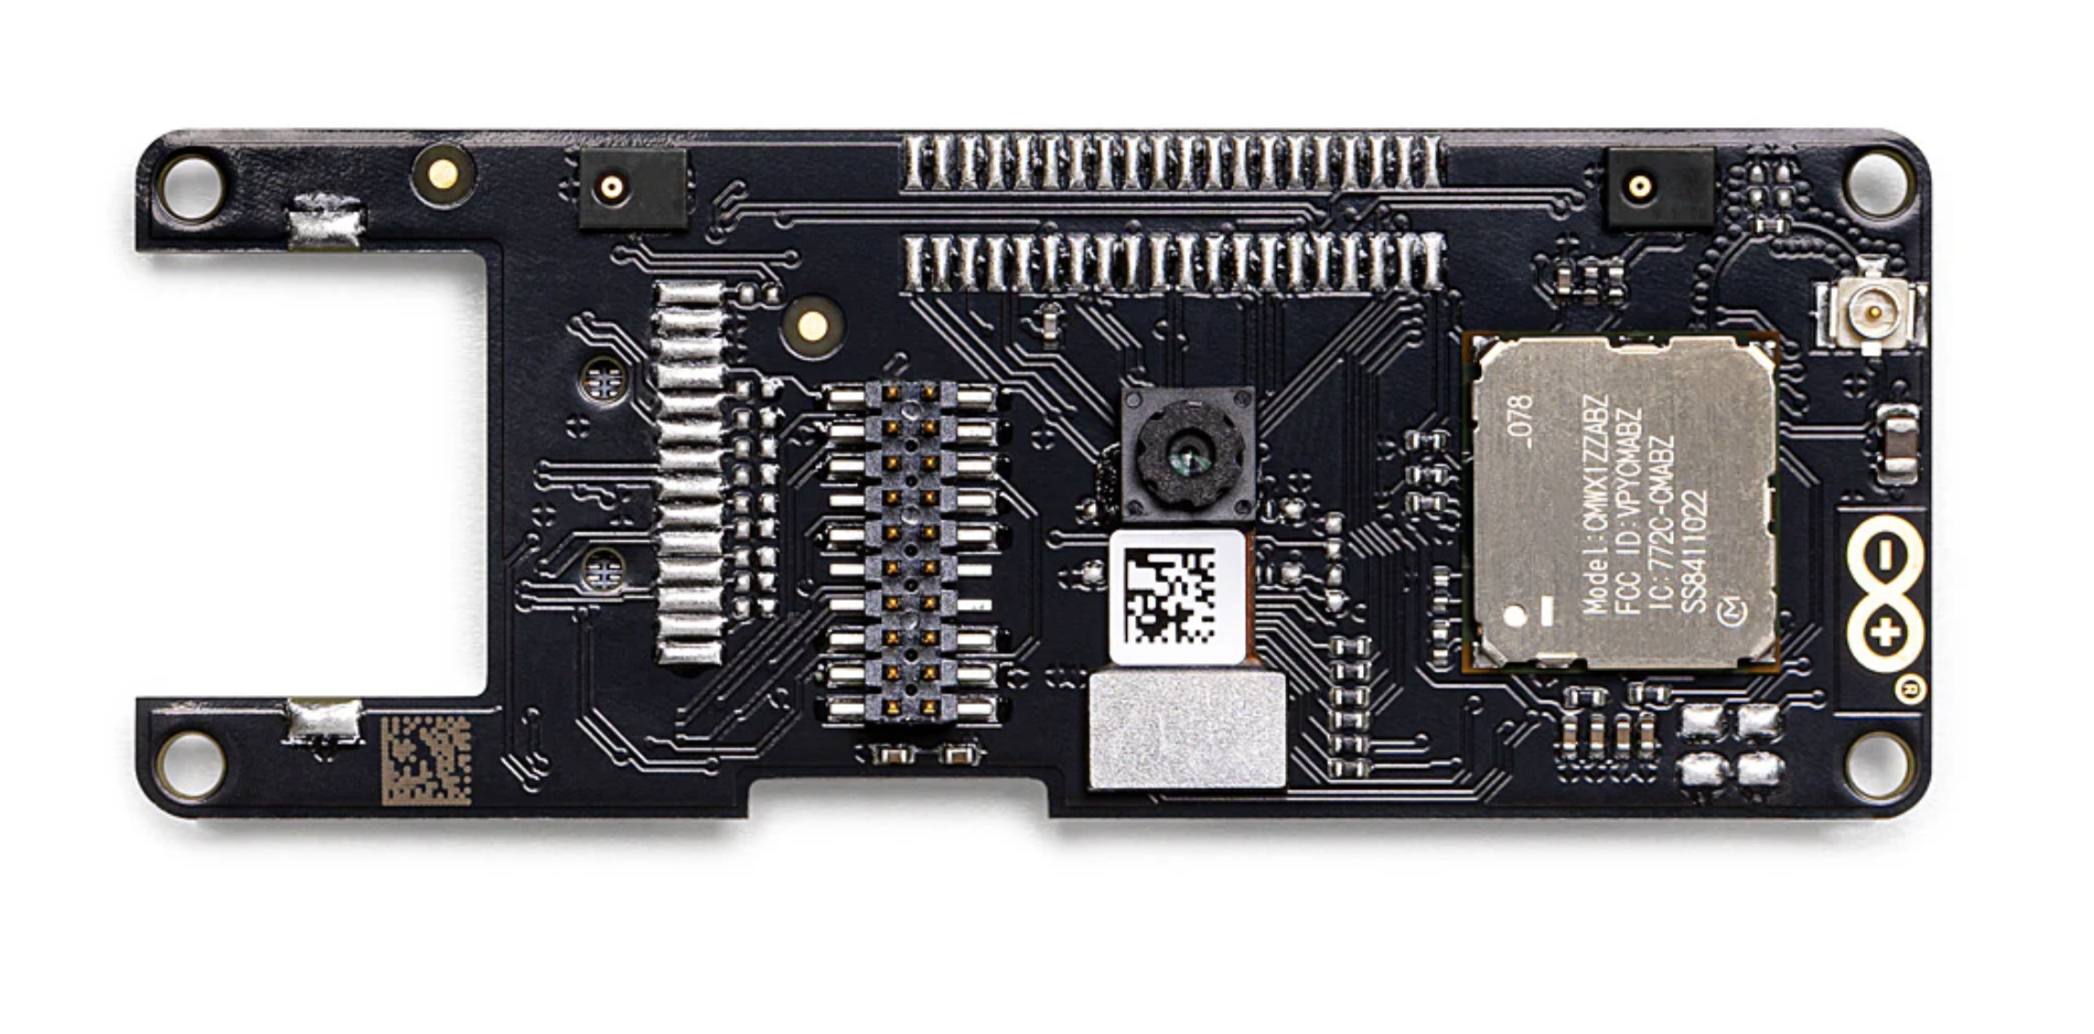
\includegraphics[width=\textwidth]{images/PortentaVisionShield.png}
			\vspace{0.2cm}
			\textbf{Figure2: PortentaH7 Vision Shield}
		\end{columns}
		
	\end{frame}
	
	\begin{frame}
		\frametitle{1. The Basic Setup:}
		
		\begin{itemize}
			\item {a. Connect the Portenta Vision Shield to your Portenta H7 as shown in the figure. The top and bottom high density connecters are connected to the corresponding ones on the underside of the H7 board. Plug in the H7 to your computer using the USB-C® cable.}
			
				\begin{columns}
					\column{0.5\textwidth}
					\centering
					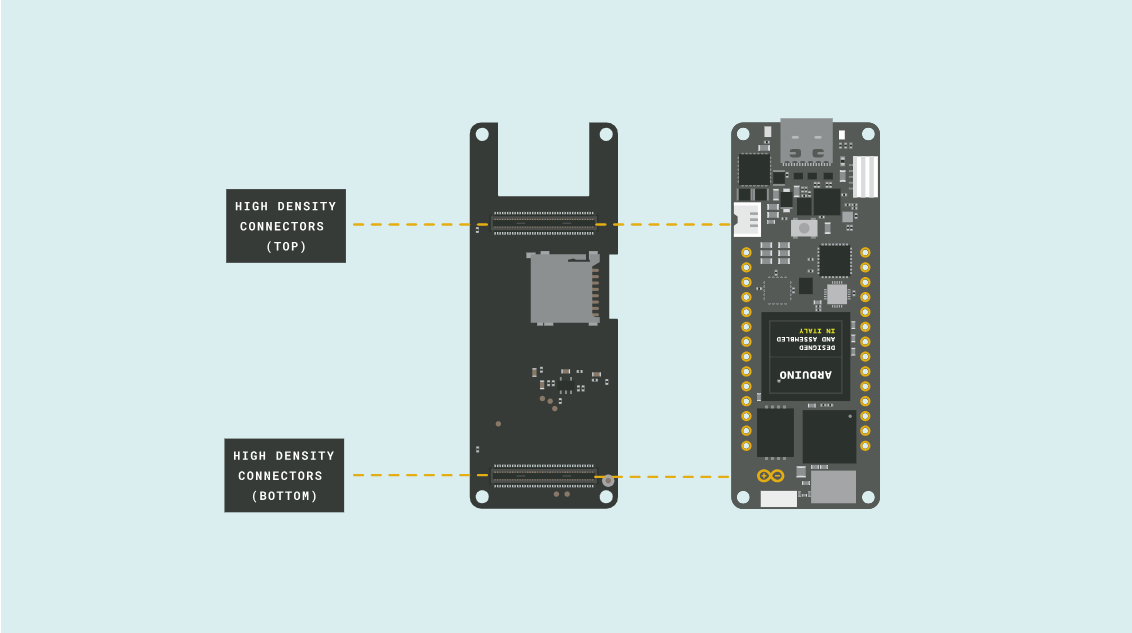
\includegraphics[width=\textwidth]{images/Connection VS.png}
					\vspace{0.2cm}
					\textbf{Figure3: Connection VS}
				\end{columns}
				
		\end{itemize}
	\end{frame}
	
		\newpage
		
	\begin{frame}
		
		\begin{itemize}
			
			\item {b. Open the board manager in the Arduino IDE and install the latest version of the Portenta Core which is v1.3.2}
				
				\begin{columns}
					\column{0.5\textwidth}
					\centering
					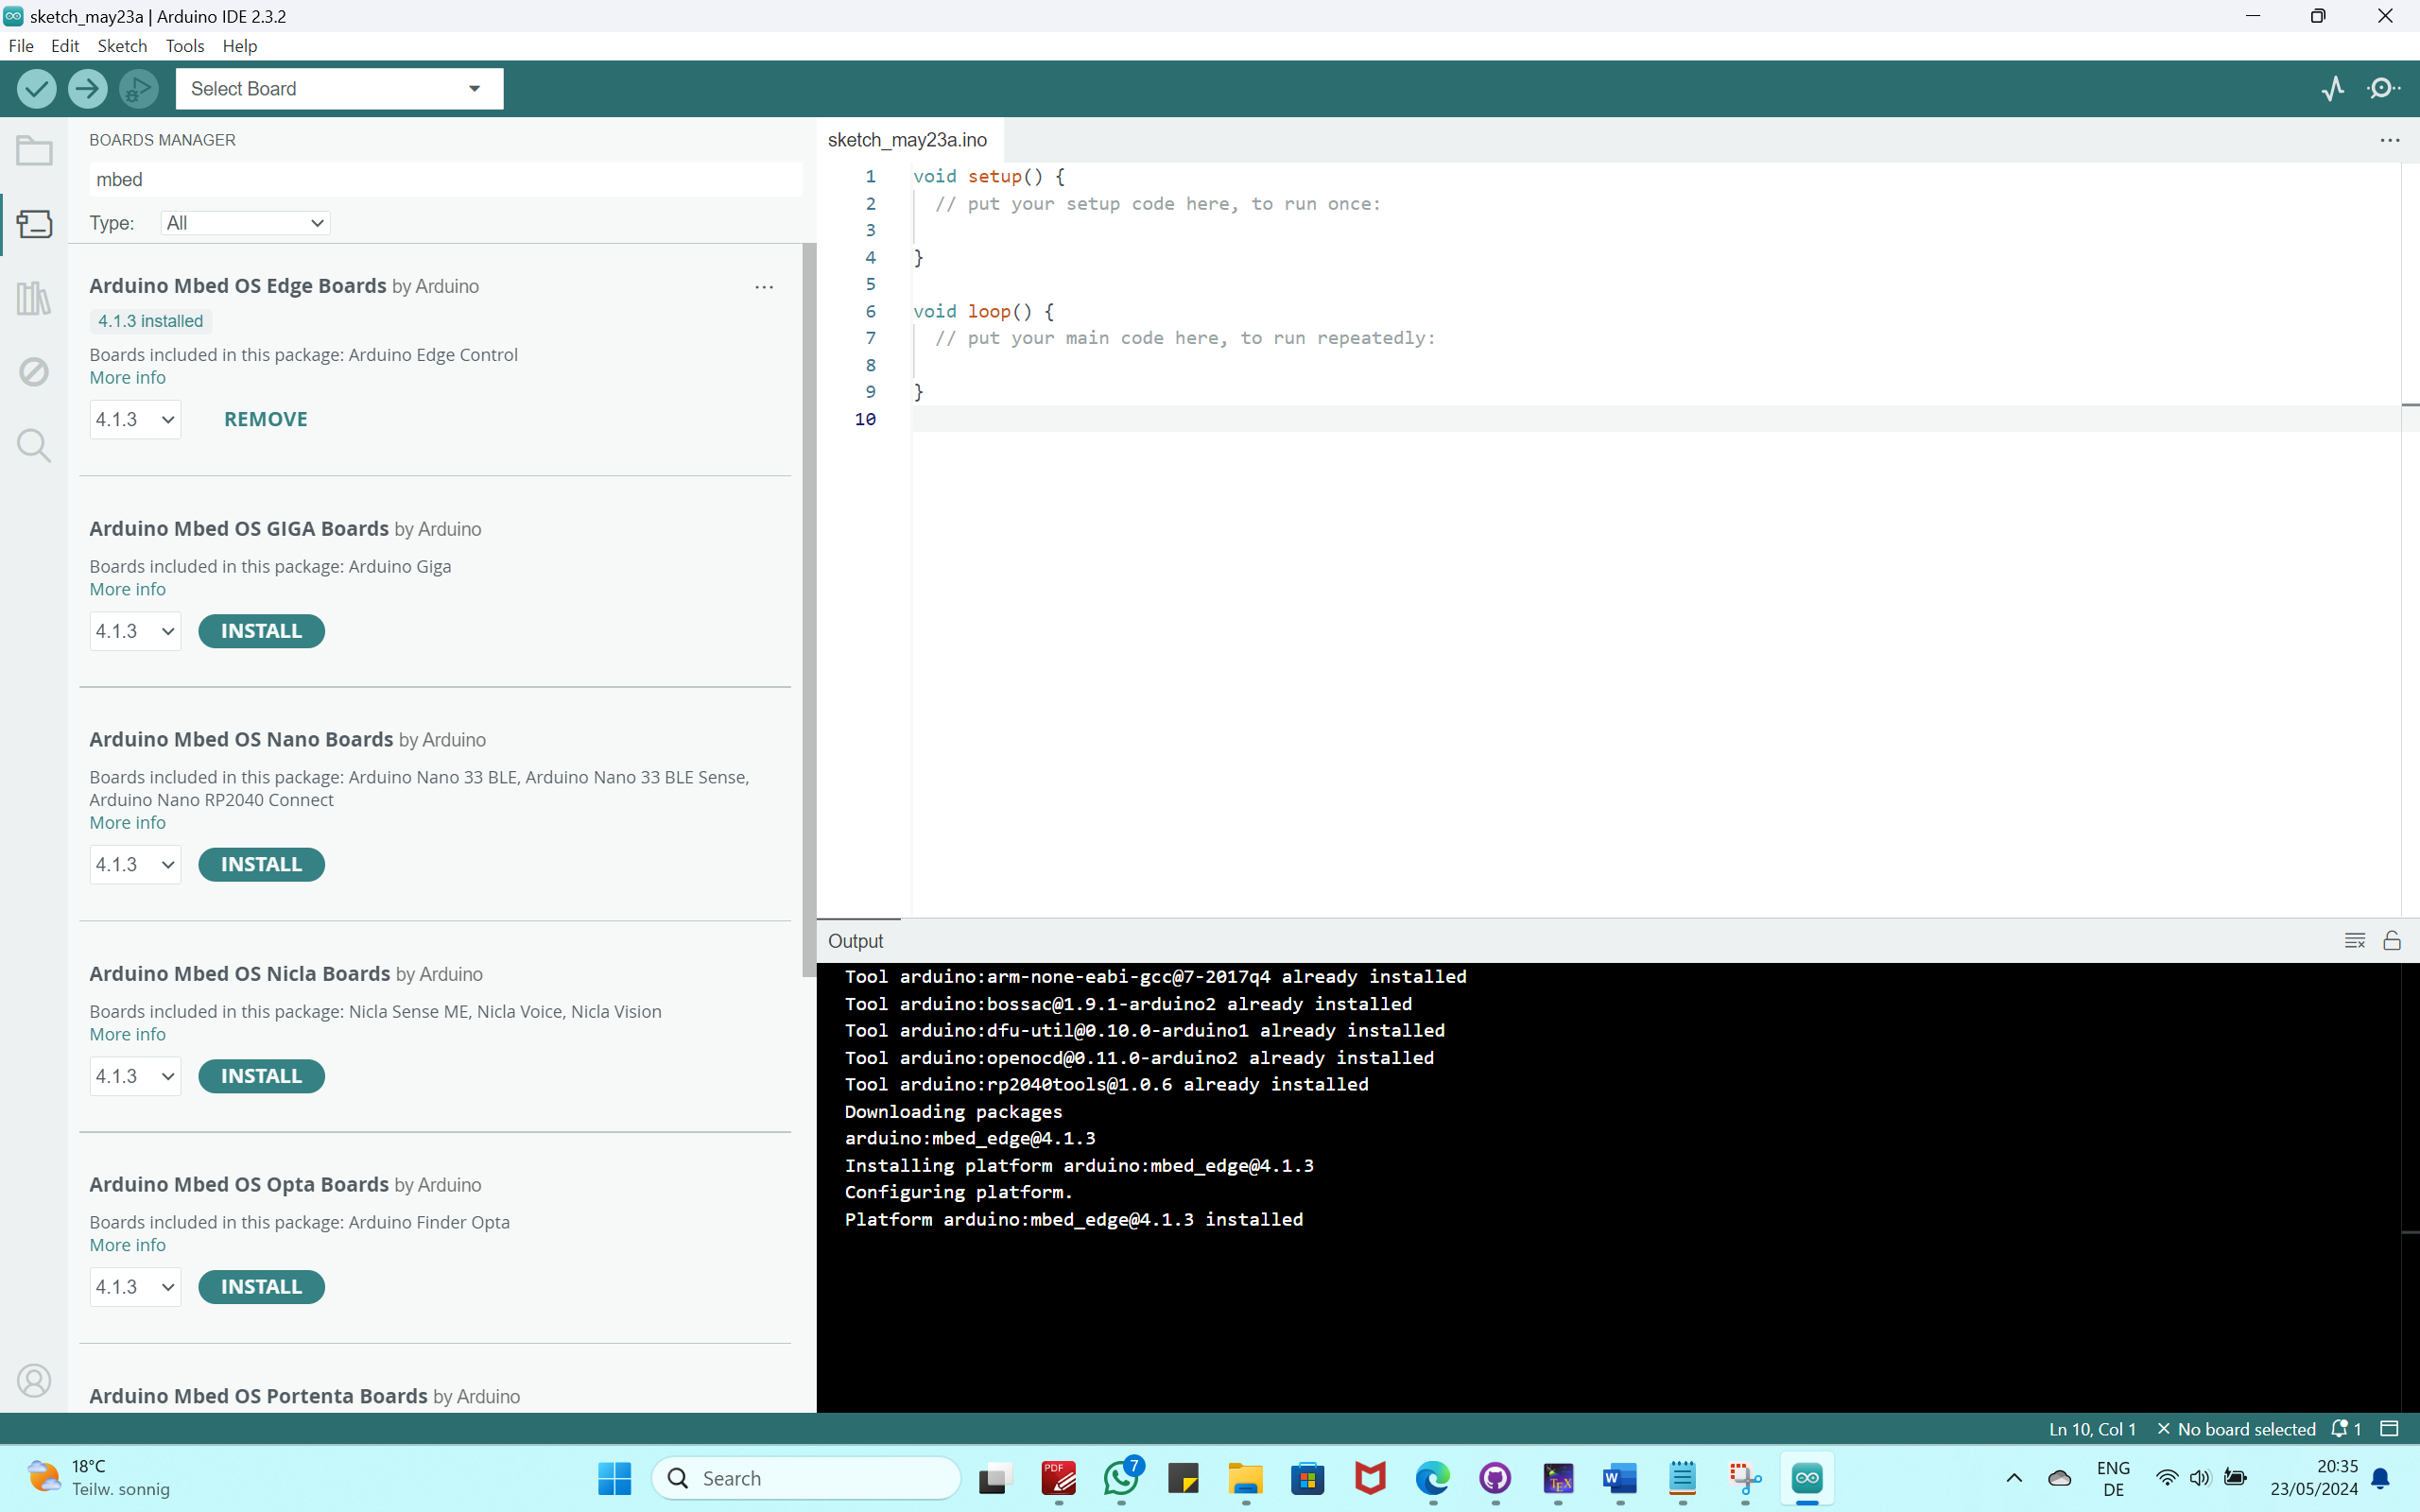
\includegraphics[width=\textwidth]{images/Portenta Core.png}
					\vspace{0.2cm}
					\textbf{Figure4: Installation}
				\end{columns}
			
		\end{itemize}
	\end{frame}
	
	\begin{frame}
		\frametitle{2. Capturing the Frames}
					
				\begin{block}{}
					Create a new Arduino sketch called CameraCapture.ino.\newline
					
					To capture the frames you will need to use the functions contained in \textbf{camera.h} which comes with the Portenta core. This library contains all APIs related to frame capturing, motion detection and pattern recognition. Include the header file in your sketch.
					content...
					
						\begin{columns}
							\column{0.5\textwidth}
							\centering
							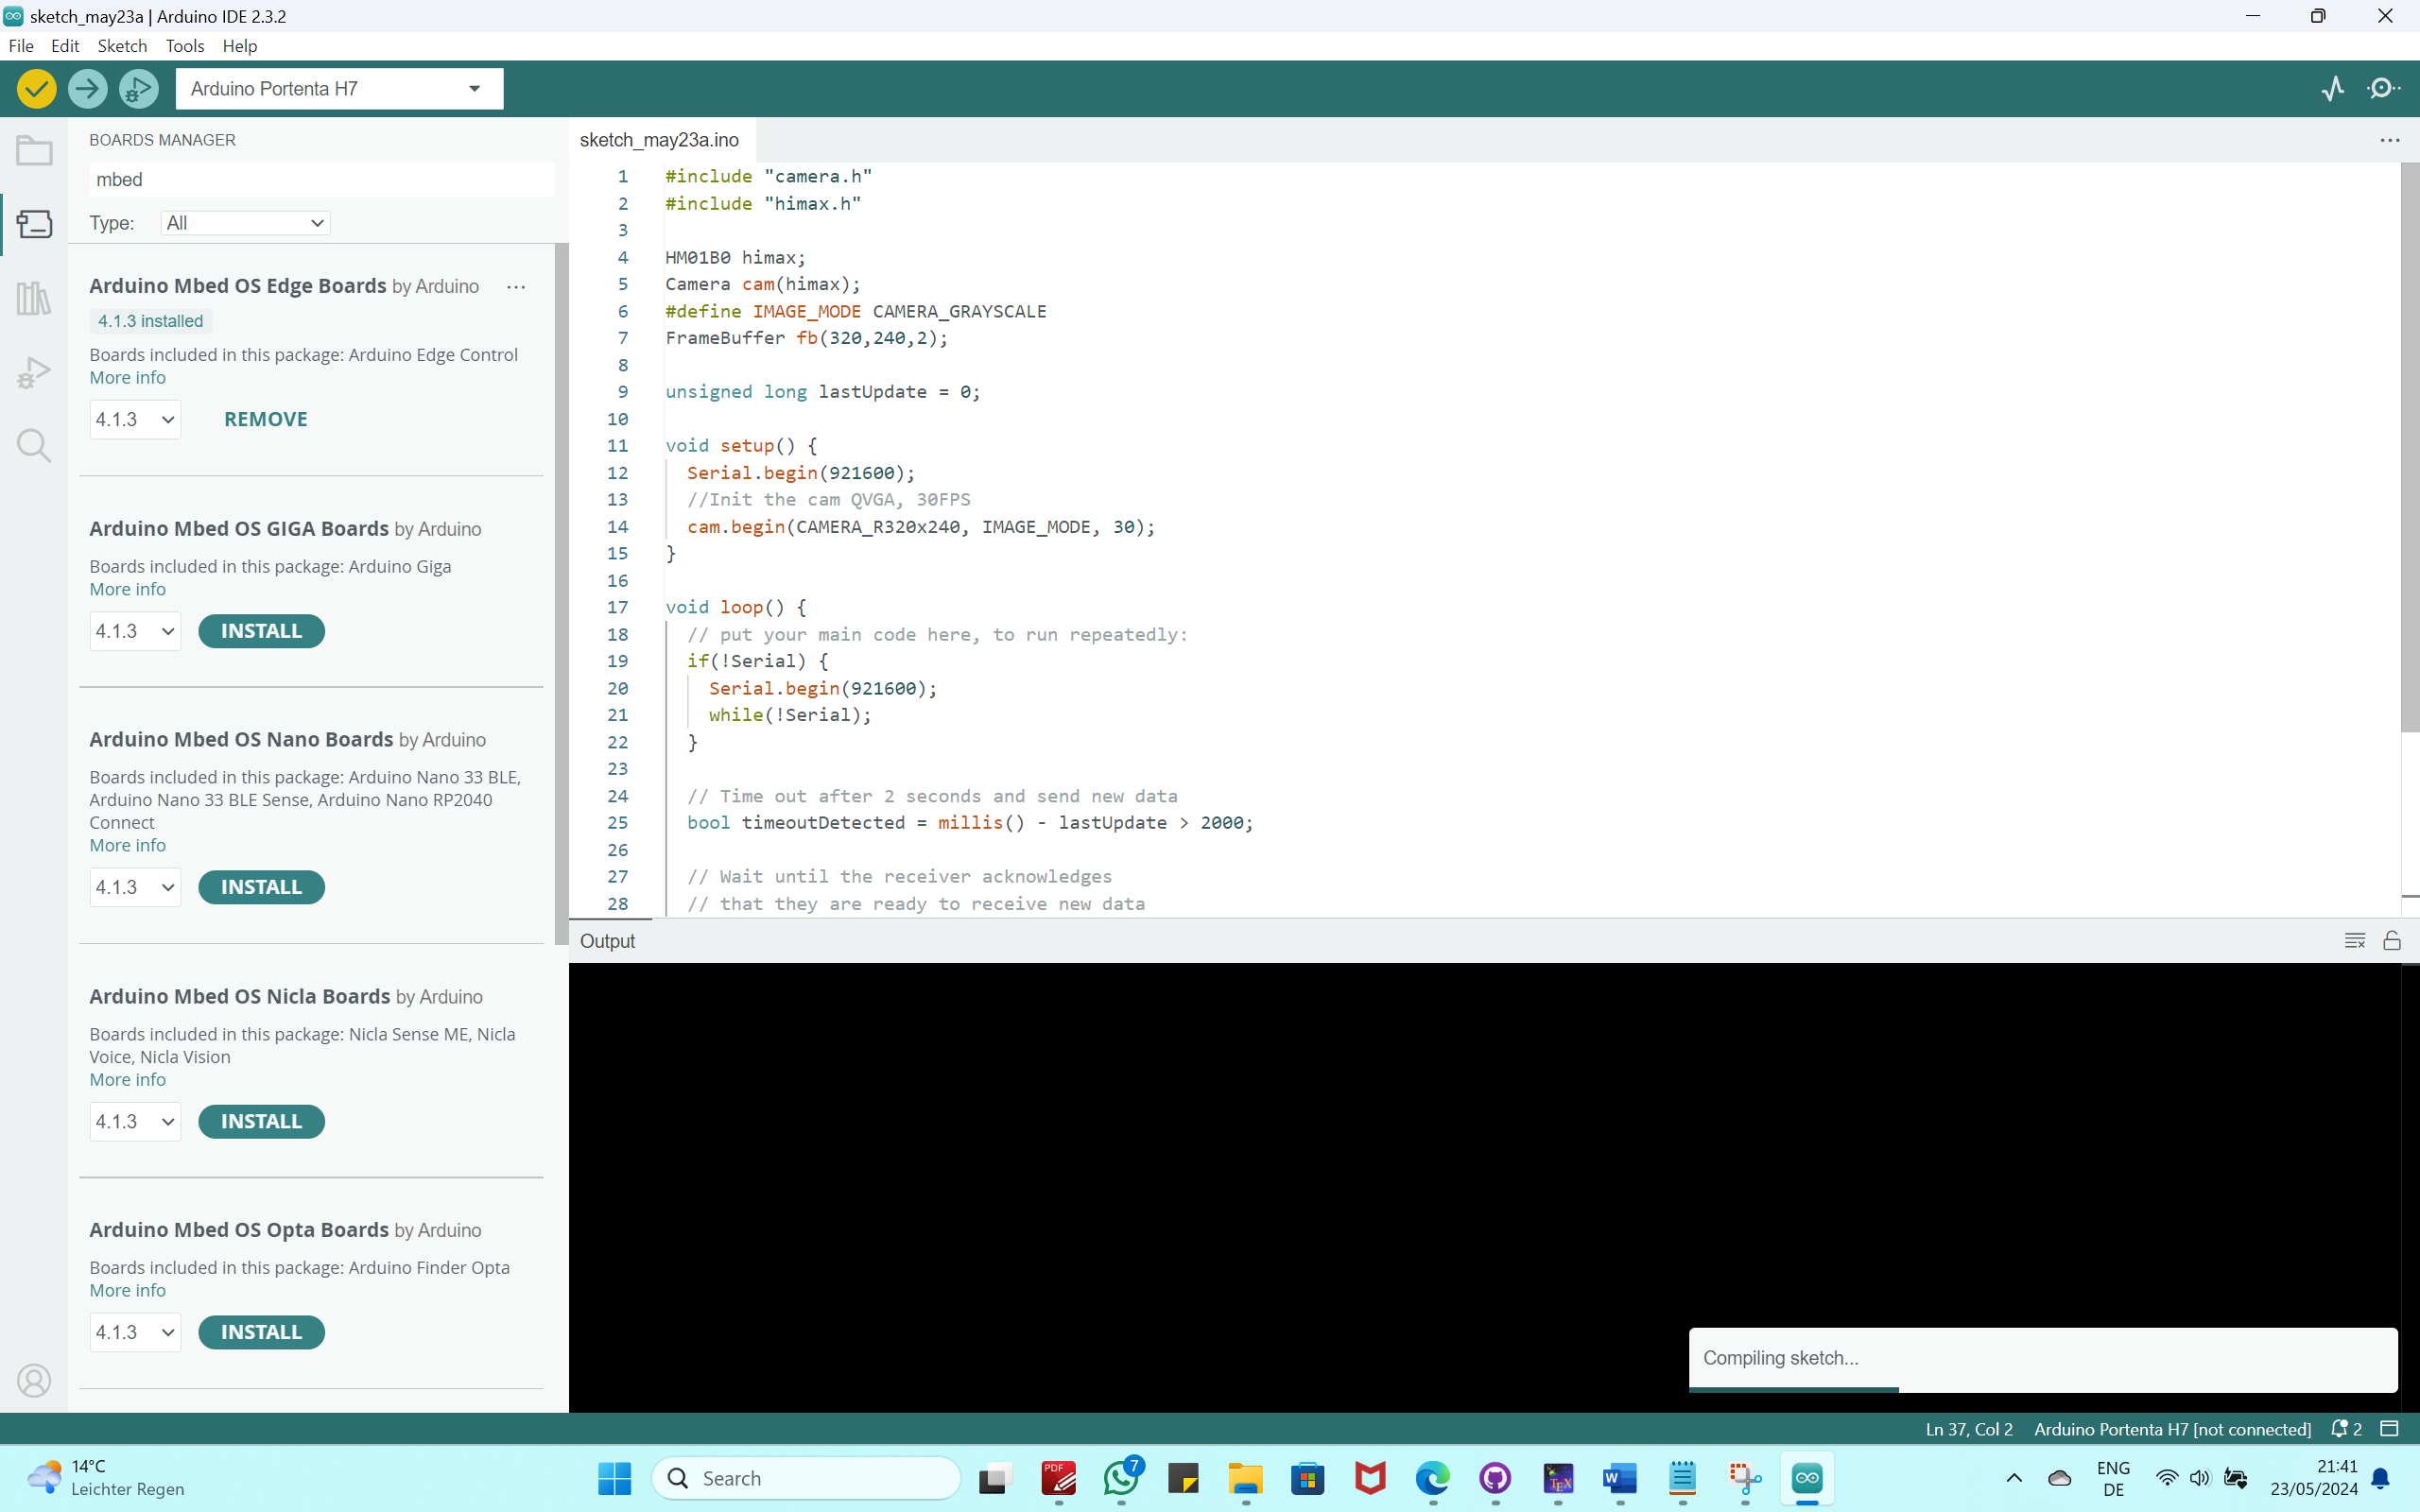
\includegraphics[width=\textwidth]{images/Testing Code.png}
							\vspace{0.2cm}
							\textbf{Figure5: Compiling}
						\end{columns}
				\end{block}
			
	\end{frame}
	
	\begin{frame}[fragile]
		\frametitle{Capture.ino}
		\begin{lstlisting}
			#include "camera.h"
			#include "himax.h"
			
			HM01B0 himax;
			Camera cam(himax);
			#define IMAGE_MODE CAMERA_GRAYSCALE
			FrameBuffer fb(320,240,2);
			
			unsigned long lastUpdate = 0;
			
			void setup() {
				Serial.begin(921600);
				//Init the cam QVGA, 30FPS
				cam.begin(CAMERA_R320x240, IMAGE_MODE, 30);
			}
			
			void loop() {
				// put your main code here, to run repeatedly:
				if(!Serial) {    
					
		\end{lstlisting}
	\end{frame}
		
	\begin{frame}[fragile]
		\frametitle{Continue...}
		\begin{lstlisting}
			Serial.begin(921600);
			while(!Serial);
			}
			// Time out after 2 seconds and send new data
			bool timeoutDetected = millis() - lastUpdate > 2000;
			
			// Wait until the receiver acknowledges
			// that they are ready to receive new data
			if(!timeoutDetected && Serial.read() != 1) return;
			
			lastUpdate = millis();
			
			// Grab frame and write to serial
			if (cam.grabFrame(fb, 3000) == 0) {
				Serial.write(fb.getBuffer(), cam.frameSize());
			}
		\end{lstlisting}
	\end{frame}
	
	
	\begin{frame}
		\frametitle{Processing}
				Download the Processing software for windows
				https://processing.org/download 
				
					\begin{columns}
						\column{0.5\textwidth}
						\centering
						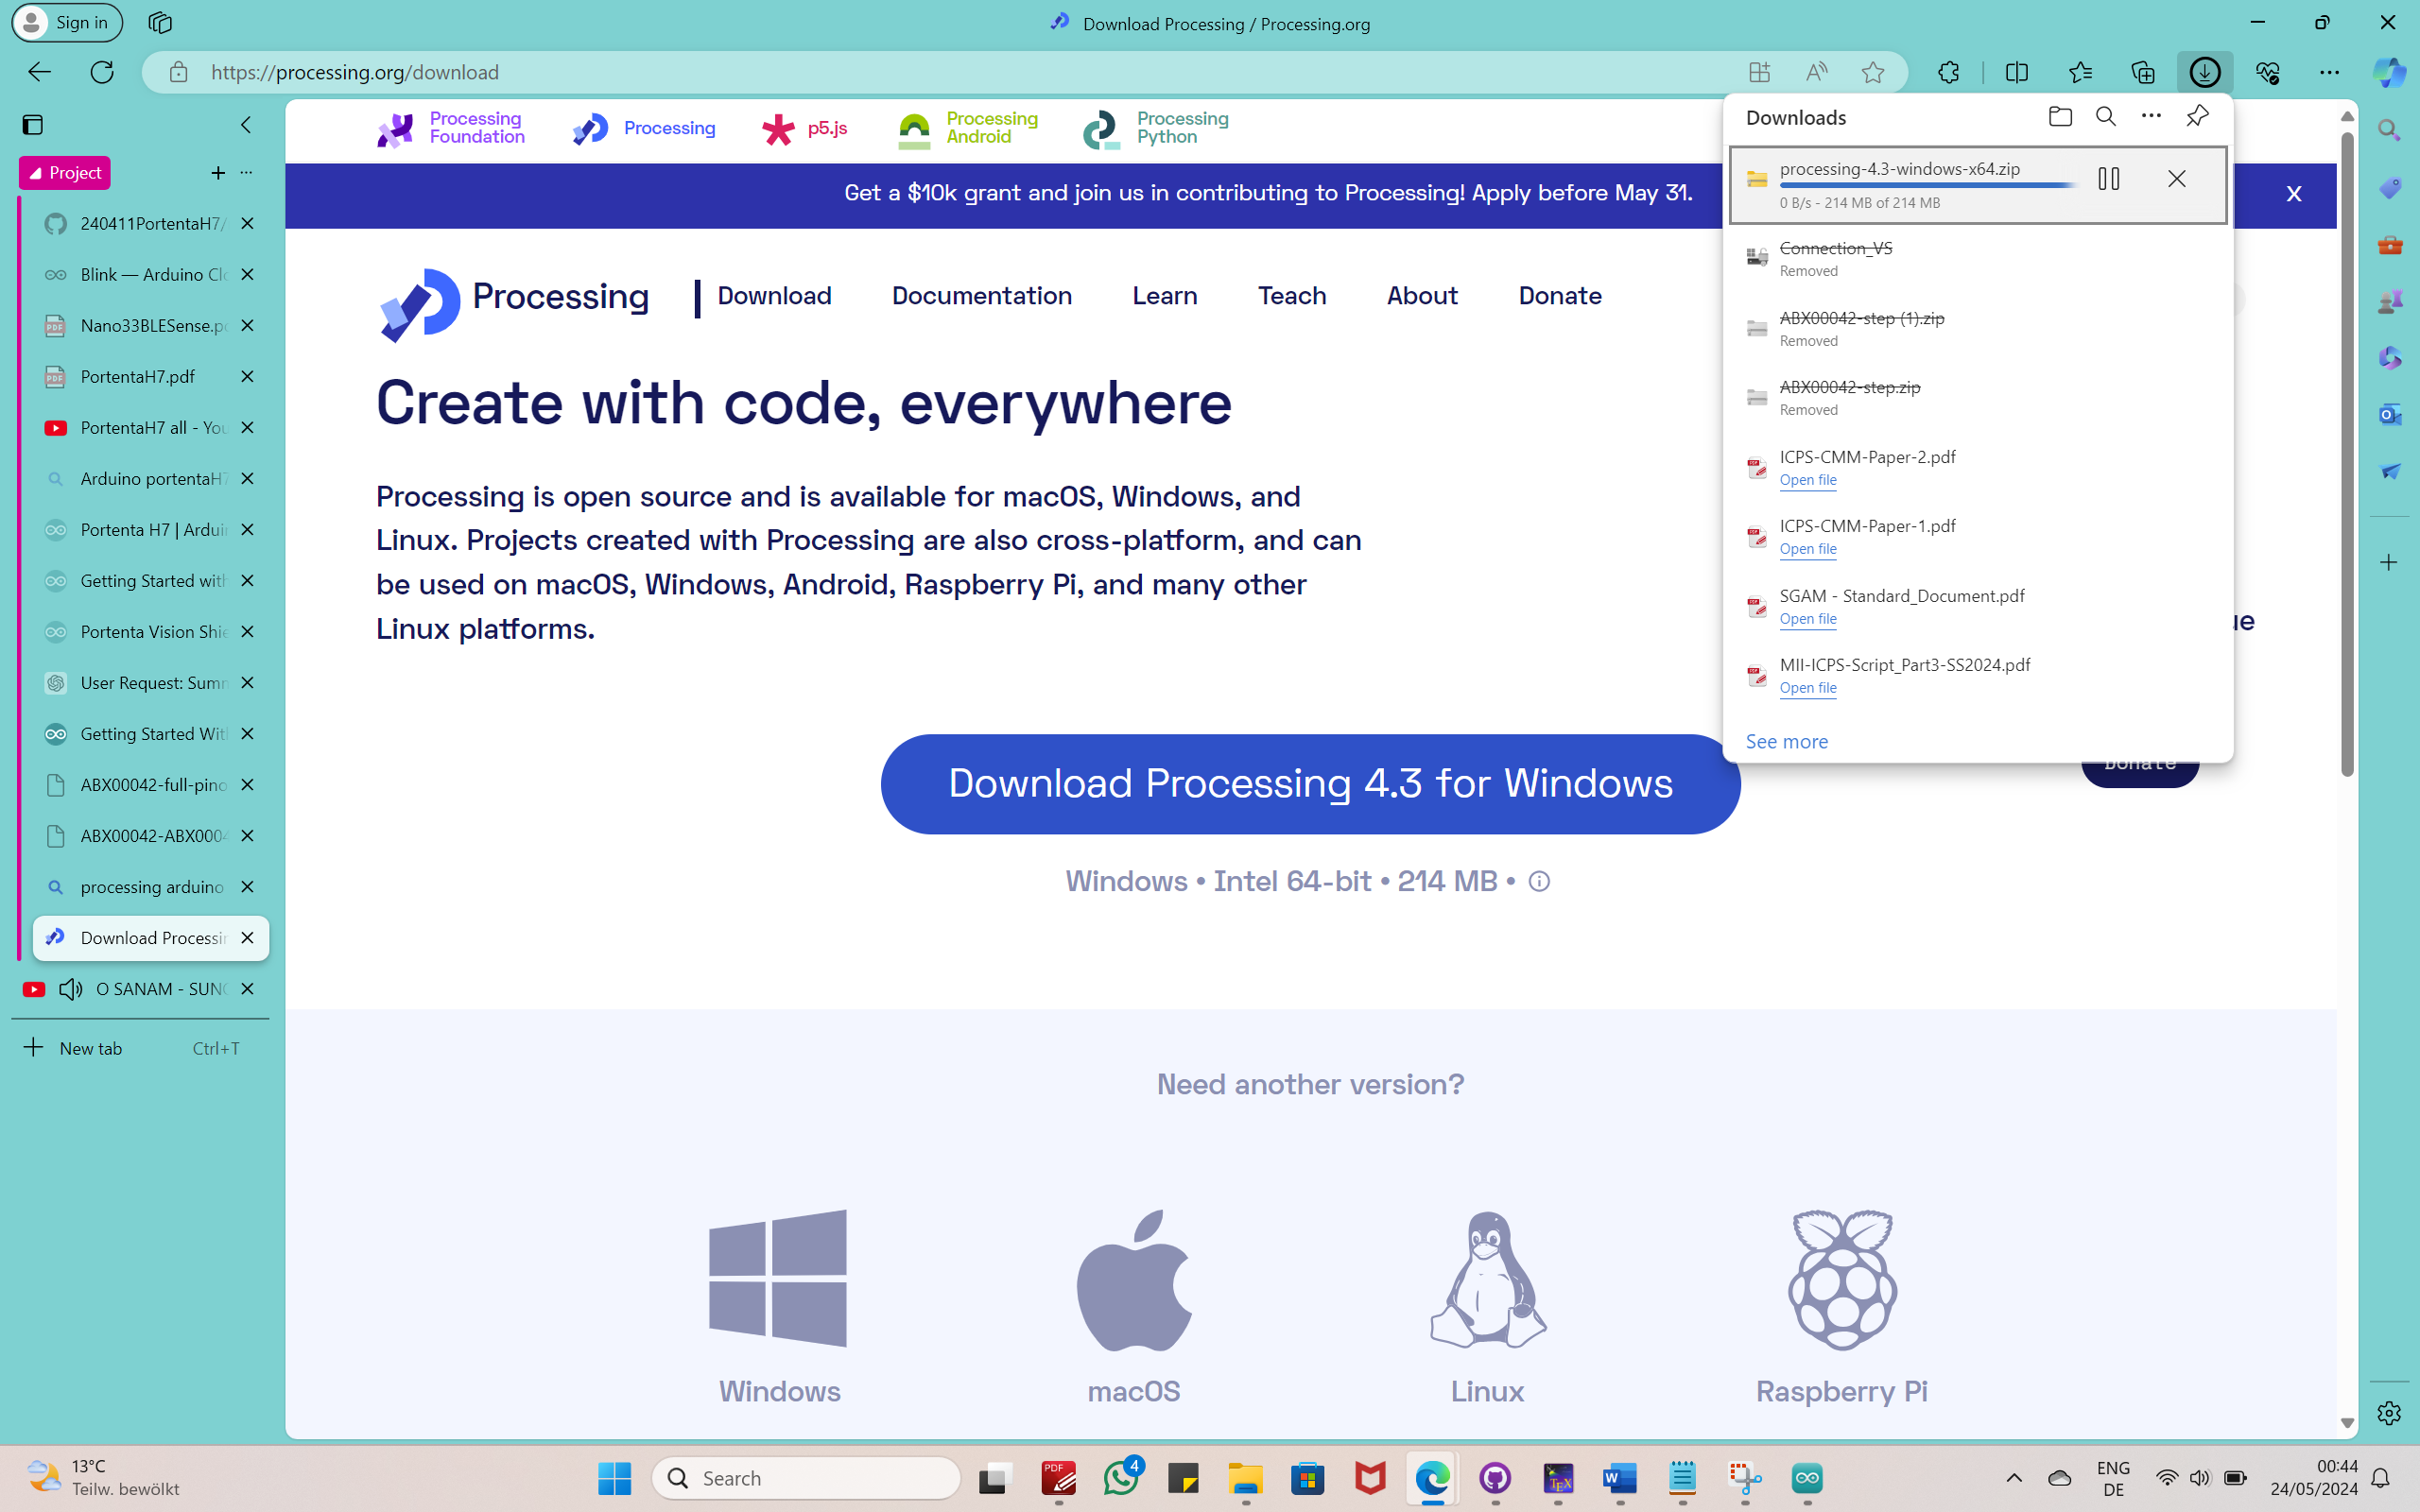
\includegraphics[width=\textwidth]{images/Download processing.png}
						\vspace{0.2cm}
						\textbf{Figure6: Downloading}
					\end{columns}
					
					\newpage
				
					\begin{columns}
						\column{0.5\textwidth}
						\centering
						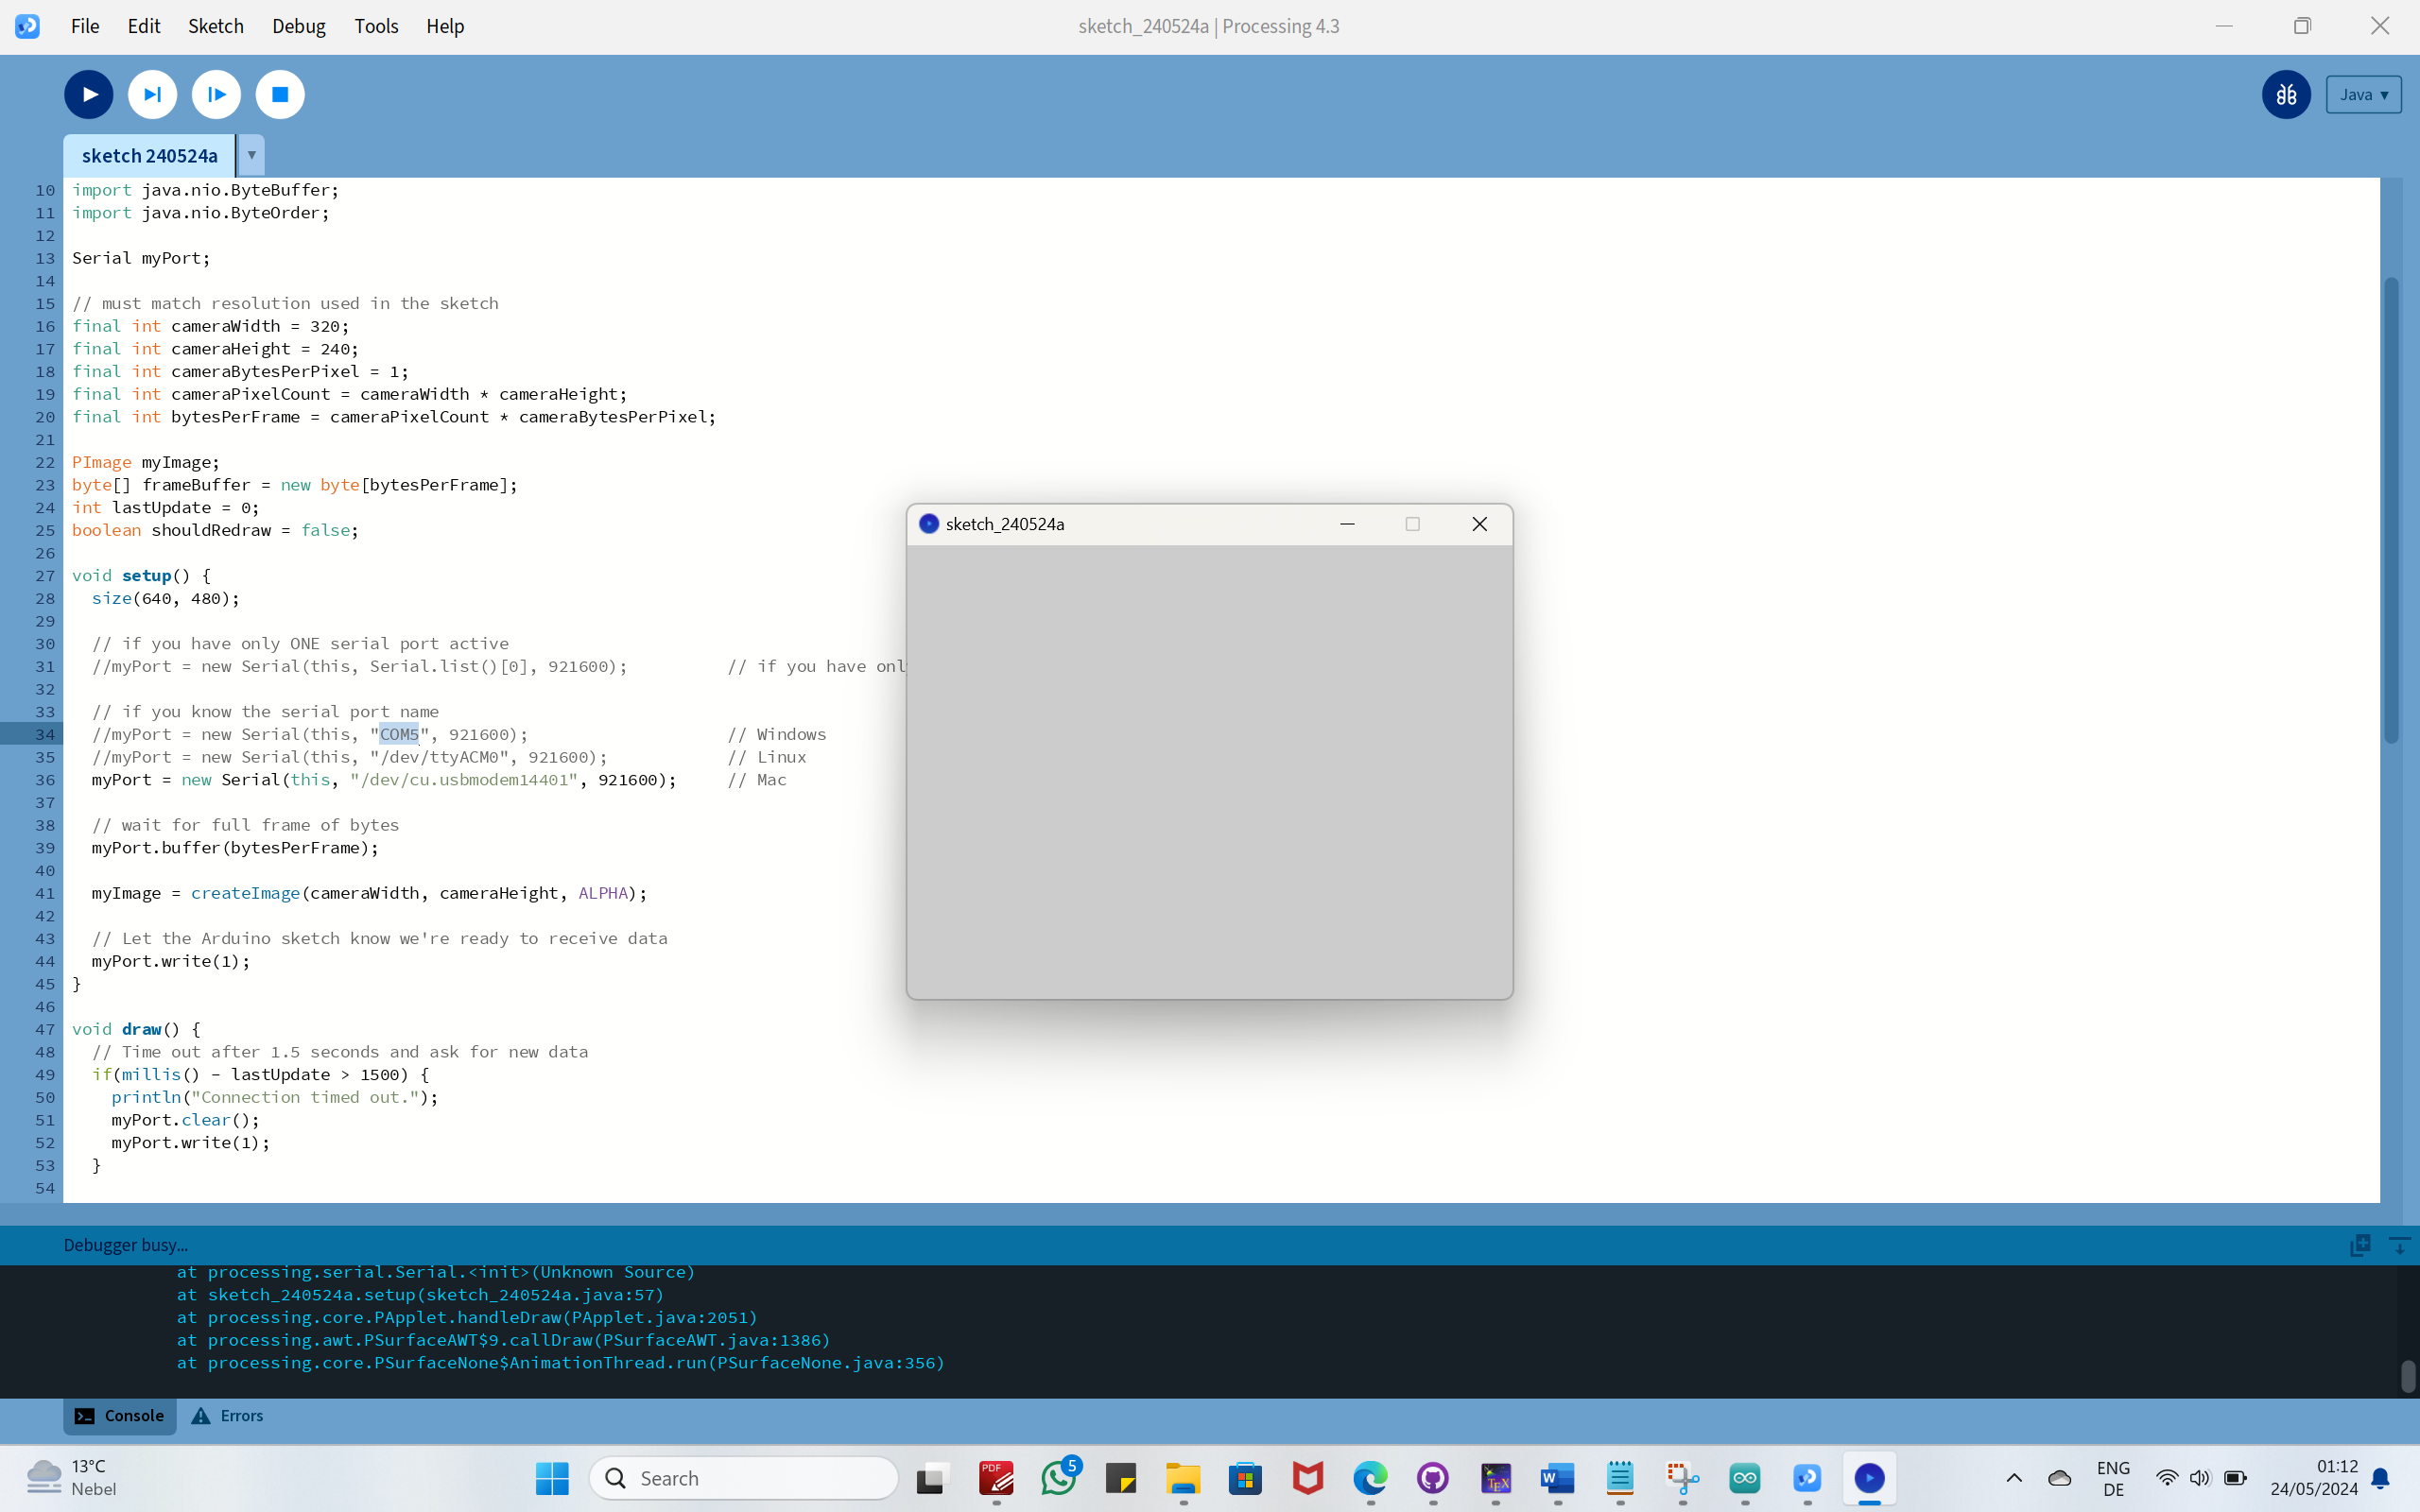
\includegraphics[width=\textwidth]{images/Execution.png}
						\vspace{0.2cm}
						\textbf{Figure6: Execution}
					\end{columns}
	
	
	\end{frame}		
	
	\begin{frame}[fragile]
		\frametitle{CameraViewer.pde}
		CODE
		\begin{lstlisting}
			/*
			import processing.serial.*;
			import java.nio.ByteBuffer;
			import java.nio.ByteOrder;
			
			Serial myPort;
			
			// must match resolution used in the sketch
			final int cameraWidth = 320;
			final int cameraHeight = 240;
			final int cameraBytesPerPixel = 1;
			final int cameraPixelCount = cameraWidth * cameraHeight;
			final int bytesPerFrame = cameraPixelCount * cameraBytesPerPixel;
			
			PImage myImage;
			byte[] frameBuffer = new byte[bytesPerFrame];
			int lastUpdate = 0;
			boolean shouldRedraw = false;
			
			void setup() {
				size(640, 480);
				
				// if you have only ONE serial port active
				//myPort = new Serial(this, Serial.list()[0], 921600);          // if you have only ONE serial port active
				
				// if you know the serial port name
				//myPort = new Serial(this, "COM5", 921600);                    // Windows
				
				// wait for full frame of bytes
				myPort.buffer(bytesPerFrame);  
				
				myImage = createImage(cameraWidth, cameraHeight, ALPHA);
				
				// Let the Arduino sketch know we're ready to receive data
				myPort.write(1);
			}
			
			void draw() {
				// Time out after 1.5 seconds and ask for new data
				if(millis() - lastUpdate > 1500) {
					println("Connection timed out.");
					myPort.clear();
					myPort.write(1);
				}
				
				if(shouldRedraw){    
					PImage img = myImage.copy();
					img.resize(640, 480);
					image(img, 0, 0);
					shouldRedraw = false;
				}
			}
			
			void serialEvent(Serial myPort) {
				lastUpdate = millis();
				
				// read the received bytes
				myPort.readBytes(frameBuffer);
				
				// Access raw bytes via byte buffer  
				ByteBuffer bb = ByteBuffer.wrap(frameBuffer);
				
				/* 
				Ensure proper endianness of the data for > 8 bit values.
				When using > 8bit values uncomment the following line and
				adjust the translation to the pixel color. 
				*/     
				//bb.order(ByteOrder.BIG_ENDIAN);
				
   
					
			\end{lstlisting}
		\end{frame}
			
			\begin{frame}[fragile]
				\frametitle{Continue...}
				\begin{lstlisting}
					int i = 0;
					
					while (bb.hasRemaining()) {
						// read 8-bit pixel
						byte pixelValue = bb.get();
						
						// set pixel color
						myImage.pixels[i++] = color(Byte.toUnsignedInt(pixelValue));    
					}
					
					myImage.updatePixels();
					
					// Ensures that the new image data is drawn in the next draw loop
					shouldRedraw = true;
					
					// Let the Arduino sketch know we received all pixels
					// and are ready for the next frame
					myPort.write(1);
					} 
			\end{lstlisting}
		\end{frame}
	
	\begin{frame}		
		\frametitle{Upload the Sketch}
			Select the right serial port on your IDE and upload the Arduino sketch to your Portenta H7. After a successful upload, run the CameraViewer.pde sketch in Processing. You should be able to see the rendered camera output on the Processing canvas.		
				\begin{columns}
					\column{0.5\textwidth}
					\centering
					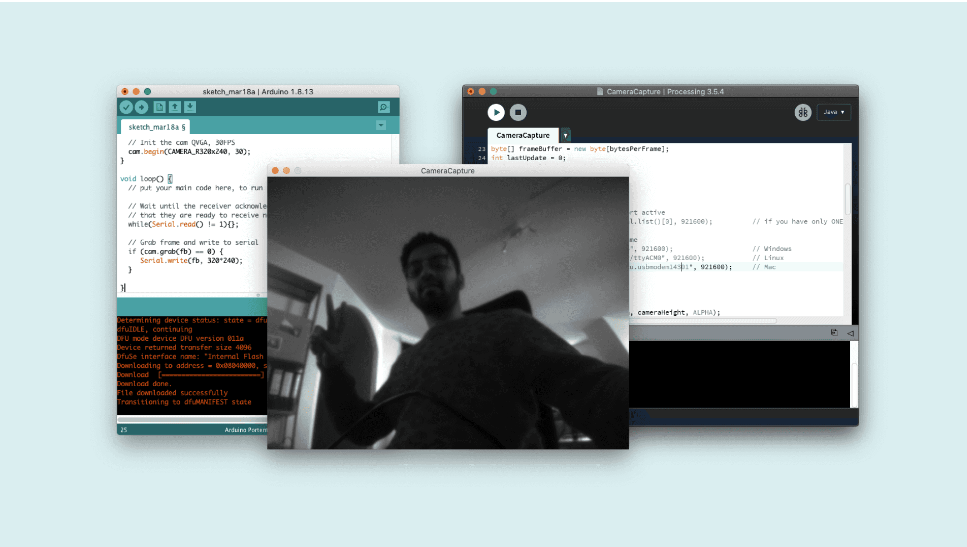
\includegraphics[width=\textwidth]{images/Camera Output.png}
					\vspace{0.2cm}
					\textbf{Figure8: Camera Output}
				\end{columns}

	\end{frame}
		
	
	\section{Applications}
	\begin{frame}
		\frametitle{Applications}
		
		Real-time object detection with the Arduino Portenta H7 and Vision Shield has numerous applications across various industries:
		
		\begin{itemize}
			\item \textbf{Surveillance and Security Systems:} Enhance security measures by detecting and identifying intruders or suspicious objects in real-time.
			\item \textbf{Industrial Automation and Quality Control:} Ensure product quality by identifying defects or anomalies on manufacturing lines.
			\item \textbf{Robotics and Autonomous Navigation:} Enable robots and autonomous vehicles to perceive and react to their surroundings, enhancing safety and efficiency.
			\item \textbf{Smart Home Devices and IoT Applications:} Create intelligent devices capable of recognizing and responding to human activities or environmental changes.
		\end{itemize}
		
		Real-time object detection provides valuable insights and automation capabilities in diverse fields, making it a versatile and powerful technology for modern applications.
		
	\end{frame}
	
	
	\section{Conclusion}
	\begin{frame}
		\frametitle{Conclusion}
		
		
		\begin{itemize}
			\item The project showcases the potential of Arduino vision shield
			\item By leveraging the computational power of the Arduino Portenta H7 and the image processing capabilities of the Vision Shield, complex tasks like object detection can be performed efficiently and accurately in real-time.
			\item The project opens up possibilities for a wide range of applications in industries such as surveillance, industrial automation, robotics, and IoT, where real-time object detection is crucial for decision-making and automation.
		\end{itemize}
		
	\end{frame}
	
	\section{Future Work}
	\begin{frame}
		\frametitle{Future Work}
		\begin{itemize}
			\item After discussion with Peers
		\end{itemize}
	\end{frame}
	
	\STANDARD{}
{
  \begin{columns}
    \begin{column}{0.35\textwidth}
      \begin{block}{~~~~~~Thank you}
        \centering
        for your attention
      \end{block}
    \end{column}
  \end{columns}
}

\MYNOTE{Ja, \textbf{Vielen} Dank, für Ihre Aufmerksamkeit}


	
\end{document}
